\subsection{K-NN on Big Data}
The K-NN algorithm can be seen to be approximately linear on figure \ref{fig:predictionTimeVStrainSize}.
It takes approximately 0.47 seconds to predict a single value.

\begin{figure}[H]
\centering
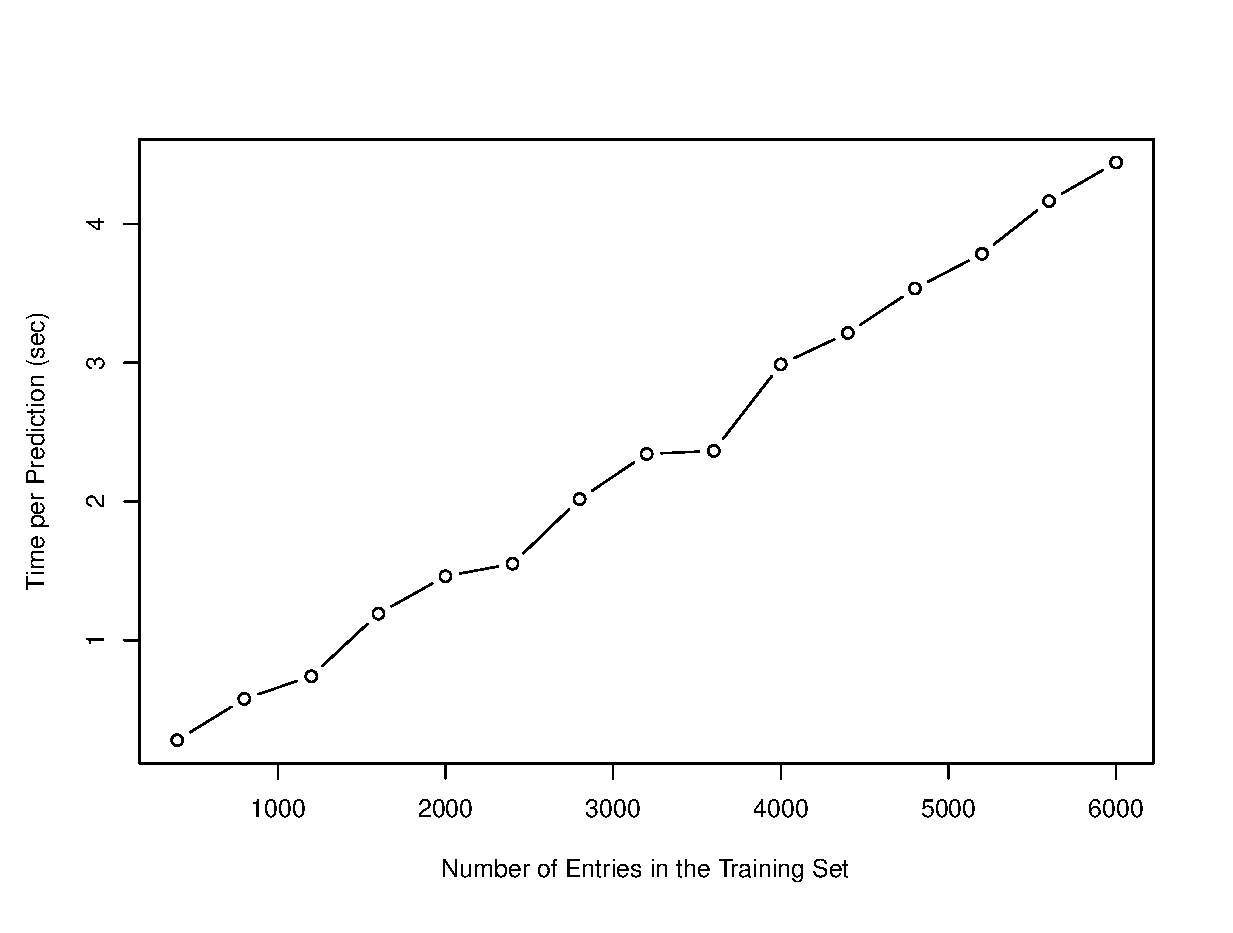
\includegraphics[width = 0.95 \textwidth]{graphics/graph_timeVSppl}
\caption{The time taken for one prediction for different training set sizes at 100 DPI resolution.}
\label{fig:predictionTimeVStrainSize}
\end{figure}

This can, when a lot of values, such as the 4000 elements dataset of a single person, take a long time to predict all of them (approx. 30 min on 100 DPI).
It is therefore desirable to bring down the prediction time.
This will be considered in the following chapters.
